\documentclass[journal,13pt,twocolumn]{IEEEtran}

\usepackage{setspace}
\usepackage{gensymb}
\counterwithin{equation}{section}
\singlespacing

\newcommand{\myvec}[1]{\ensuremath{\begin{pmatrix}#1\end{pmatrix}}}
\newcommand{\mydet}[1]{\ensuremath{\begin{vmatrix}#1\end{vmatrix}}}

\usepackage[cmex10]{amsmath}
\usepackage{amsthm}
\usepackage{mathrsfs}
\usepackage{txfonts}
\usepackage{stfloats}
\usepackage{bm}
\usepackage{cite}
\usepackage{cases}
\usepackage{subfig}
\usepackage{longtable}
\usepackage{multirow}
\usepackage{mathtools}
\usepackage{steinmetz}
\usepackage{tikz}
\usepackage{circuitikz}
\usepackage{verbatim}
\usepackage{tfrupee}
\usepackage[breaklinks=true]{hyperref}
\usepackage{tkz-euclide} % loads  TikZ and tkz-base
%\usetkzobj{all}
\usetikzlibrary{calc,math}
\usepackage{listings}
    \usepackage{color}                                            %%
    \usepackage{array}                                            %%
    \usepackage{longtable}                                        %%
    \usepackage{calc}                                             %%
    \usepackage{multirow}                                         %%
    \usepackage{hhline}                                           %%
    \usepackage{ifthen}                                           %%
  %optionally (for landscape tables embedded in another document): %%
    \usepackage{lscape}     
\usepackage{multicol}
\usepackage{chngcntr}
\usepackage{pgfplots}
\usepackage{pgfplotstable}
\pgfplotsset{compat=1.7}
\usepackage{tikz}
\DeclareMathOperator*{\Res}{Res}
\renewcommand\thesection{\arabic{section}}
\renewcommand\thesubsection{\thesection.\arabic{subsection}}
\renewcommand\thesubsubsection{\thesubsection.\arabic{subsubsection}}

\renewcommand\thesectiondis{\arabic{section}}
\renewcommand\thesubsectiondis{\thesectiondis.\arabic{subsection}}
\renewcommand\thesubsubsectiondis{\thesubsectiondis.\arabic{subsubsection}}

\DeclarePairedDelimiter\abs{\lvert}{\rvert} % \abs{} for numerisk værdi
\DeclarePairedDelimiter\norm{\lVert}{\rVert}
\makeatletter
\let\oldabs\abs
\def\abs{\@ifstar{\oldabs}{\oldabs*}}
\let\oldnorm\norm
\def\norm{\@ifstar{\oldnorm}{\oldnorm*}}
\makeatother
\renewcommand{\vec}[1]{\mathbf{#1}}
\newcommand{\bignorm}[1]{\Bigl \| #1 \Bigr \| #1}
\hyphenation{op-tical net-works semi-conduc-tor}
\def\inputGnumericTable{}                                 %%

\lstset{
frame=single, 
breaklines=true,
columns=fullflexible
}
\begin{document}
\title{Assignment 4} 
\author{Shweta Verma} 
\maketitle
\newpage
\bigskip
\begin{abstract}
This document determines the value of $k$ for which the given equation represents a pair of straight lines.
\end{abstract}
\section{\textbf{Problem}}
For what value of $k$ does the equation 
\begin{align}
\vec{x}^T \myvec{6 && k/2 \\ k/2 && -3} \vec{x} + \myvec{4 && 5}\vec{x} -2 = 0
\end{align}
represent a pair of straight lines?
\section{\textbf{Solution}}
Equation (1.1) can also be written as 
\begin{align}
\vec{x}^T \myvec{a && b \\ b && c} \vec{x} + \myvec{d && e}\vec{x} + f = 0
\end{align}
\begin{equation}
\begin{split}
\vec{V}=\myvec{6 && k/2\\ k/2 && -3}\\
\vec{u}=\myvec{2\\5/2}\\
f= -2
\end{split}
\end{equation}
Block Matrix
\begin{align}
 = \myvec{6 && k/2 && 2\\ k/2 && -3 && 5/2\\2 && 5/2 && -2}
\end{align}
Determinant of the Block Matrix
\begin{align}
\Delta = \mydet{6 && k/2 && 2\\ k/2 && -3 && 5/2\\2 && 5/2 && -2}
\end{align}
If the equation (1.1) represents a pair of straight lines\\
then the Determinant is zero
\begin{align}
\Delta = 0
\end{align}
\begin{align}
\implies \mydet{6 && k/2 && 2\\ k/2 && -3 && 5/2\\2 && 5/2 && -2} = 0
\end{align}
\begin{align}
\implies 6\times(6-25/4)-k/2(-k-5)+2(5k/4+6) = 0
\end{align}
\begin{align}
\implies k^2 + 10k + 21 = 0
\end{align}
\begin{align}
\implies \boxed{ k = -3 }
\end{align}
\begin{align}
\implies \boxed{ k = -7 }
\end{align}
Substituting k=-3 in (1.1)
\begin{align}
\vec{x}^T \myvec{6 && -3/2 \\ -3/2 && -3} \vec{x} + \myvec{4 && 5}\vec{x} -2 = 0
\end{align}
Equation (2.2) can be represented as 
\begin{equation}
\begin{split}
\vec{V}=\myvec{6 && -3/2\\ -3/2 && -3}\\
\vec{u}=\myvec{2\\5/2}\\
f= -2
\end{split}
\end{equation}
To find the separate equations of the straight lines we will use spectral decomposition.\\
Characteristic equation of $\vec{V}$ is given by:
\begin{equation}
\begin{split}
\mydet{V-\lambda \vec{I}}=\mydet{6-\lambda && -3/2\\ -3/2 && -3-\lambda} = 0\\
\implies \lambda^2 - 3\lambda - 81/4 = 0
\end{split}
\end{equation}
The Eigen Values of $\vec{V}$ are:
\begin{align}
\lambda_1 = \frac{3+3\sqrt{10}}{2}, \lambda_2 = \frac{3-3\sqrt{10}}{2}
\end{align}
Let $\vec{p}_1$ and $\vec{p}_2$ be the Eigen vector corresponding to $\lambda_1$ and $\lambda_2$ respectively\\
Eigen vector $\vec{p}$ is given as:
\begin{equation} 
\begin{split}
\vec{V}\vec{p} = \lambda\vec{p}\\
\implies (\vec{V} - \lambda \vec{I})\vec{p} = 0
\end{split}
\end{equation}
For $\lambda_1 = \frac{3+3\sqrt{10}}{2}$
\begin{align}
(\vec{V} - \lambda_1 \vec{I}) = \myvec{\frac{9-3\sqrt{10}}{2} && -3/2\\ -3/2 && \frac{-9-3\sqrt{10}}{2}}
\end{align}
To find $ \vec{p}_1 $ Use Augmented Matrix of $(\vec{V} - \lambda \vec{I})$
\begin{equation}
\begin{split}
 \myvec{\frac{9-3\sqrt{10}}{2} && -3/2 && 0\\ -3/2 && \frac{-9-3\sqrt{10}}{2} && 0}\\
\xleftrightarrow[]{R_1\rightarrow \frac{2}{9-3\sqrt{10}}R_1} 
\myvec{1 && 3+\sqrt{10} && 0\\ -3/2 && \frac{-9-3\sqrt{10}}{2} && 0}\\
\xleftrightarrow[]{R_1\rightarrow 3/2R_1+R_2} 
\myvec{1 && 3+\sqrt{10} && 0\\ 0 && 0 && 0} 
\end{split}
\end{equation}
So we get,
\begin{align}
x_1 + (3+\sqrt{10})x_2 = 0
\end{align}
Therefore, Eigen Vector corresponding to $\lambda_1$
\begin{align}
\vec{p}_1 =\frac{1}{\sqrt{20+6\sqrt{10}}} \myvec{-(3+\sqrt{10}) \\ 1}
\end{align}
Similarly for $\lambda_2 = \frac{3-3\sqrt{10}}{2}$
\begin{align}
\vec{p}_2 =\frac{1}{\sqrt{20-6\sqrt{10}}} \myvec{-(3-\sqrt{10}) \\ 1}
\end{align}
We know that $\vec{V} = \vec{P}\vec{D}\vec{P}^T$ where $\vec{P}$ and $\vec{V}$ are given by:
\begin{align}
\vec{D} = \myvec{\lambda_1 && 0\\ 0 && \lambda_2}\\
\implies \vec{D} = \myvec{\frac{3+3\sqrt{10}}{2} && 0\\ 0 &&\frac{3-3\sqrt{10}}{2} }
\end{align}
Hence the rotation matrix P is
\begin{align}
\vec{P} = \myvec{\vec{p}_1 && \vec{p}_2}\\
\implies \vec{P} = \myvec{\frac{-(3+\sqrt{10})}{\sqrt{20+6\sqrt{10}}} && \frac{-(3-\sqrt{10})}{\sqrt{20-6\sqrt{10}}} \\ \frac{1}{\sqrt{20+6\sqrt{10}}} && \frac{1}{\sqrt{20-6\sqrt{10}}}}
\end{align}
We know that 
\begin{align}
\myvec{\sqrt{|\lambda_1|} && \sqrt{|\lambda_2|}}\vec{P}^T(\vec{x}-\vec{c}) = 0
\end{align}
where $\vec{c}$ is the point of intersection of the lines 
Let $(\alpha,\beta)$ be the point of intersection of the lines 
\begin{equation}
\begin{split}
\vec{V}\vec{c} = -\vec{u}\\
\myvec{6 && -3/2\\-3/2 && -3} \myvec{\alpha \\ \beta} = -\myvec{2 \\ 5/2}\\
\implies \myvec{\alpha \\ \beta} = \myvec{-1/9 \\ 8/9}
\end{split}
\end{equation}
Substituting values in (2.25)
\begin{equation} 
\begin{split}
\myvec{ \sqrt{\frac{3+3\sqrt{10}}{2}} && \pm\sqrt{\frac{3-3\sqrt{10}}{2}}} \times \\
\myvec{ -\frac{3+\sqrt{10}}{\sqrt{20+6\sqrt{10}}} && \frac{1}{\sqrt{20+6\sqrt{10}}} \\ -\frac{3-\sqrt{10}}{\sqrt{20-6\sqrt{10}}} && -\frac{1}{\sqrt{20-6\sqrt{10}}}} \times \\
\myvec{x+1/9 \\ y-8/9}  = 0
\end{split}
\end{equation}
Simplifying (2.27) we get 
\begin{equation}
\begin{split}
3x - 3y + 3 = 0 ~and~ 2x + y - 2/3 = 0\\
\boxed{(3x - 3y + 3)(2x + y - 2/3) = 0}
\end{split}
\end{equation}
Similarly substituting k=-7 in (1.1)
\begin{align}
\vec{x}^T \myvec{6 && -7/2 \\ -7/2 && -3} \vec{x} + \myvec{4 && 5}\vec{x} -2 = 0
\end{align}
Equation (2.2) can be represented as 
\begin{equation}
\begin{split}
\vec{V}=\myvec{6 && -7/2\\ -7/2 && -3}\\
\vec{u}=\myvec{2\\5/2}\\
f= -2
\end{split}
\end{equation}
To find the separate equations of the straight lines we will use spectral decomposition.\\
Characteristic equation of $\vec{V}$ is given by:
\begin{equation}
\begin{split}
\mydet{V-\lambda \vec{I}}=\mydet{6-\lambda && -7/2\\ -7/2 && -3-\lambda} = 0\\
\implies \lambda^2 - 3\lambda - 121/4 = 0
\end{split}
\end{equation}
The Eigen Values of $\vec{V}$ are:
\begin{align}
\lambda_1 = \frac{3+\sqrt{130}}{2}, \lambda_2 = \frac{3-3\sqrt{130}}{2}
\end{align}
Let $\vec{p}_1$ and $\vec{p}_2$ be the Eigen vector corresponding to $\lambda_1$ and $\lambda_2$ respectively\\
Eigen vector $\vec{p}$ is given as:
\begin{equation} 
\begin{split}
\vec{V}\vec{p} = \lambda\vec{p}\\
\implies (\vec{V} - \lambda \vec{I})\vec{p} = 0
\end{split}
\end{equation}
For $\lambda_1 = \frac{3+\sqrt{130}}{2}$
\begin{align}
(\vec{V} - \lambda_1 \vec{I}) = \myvec{\frac{9-\sqrt{130}}{2} && -7/2\\ -7/2 && \frac{-9-\sqrt{130}}{2}}
\end{align}
To find $ \vec{p}_1 $ Use Augmented Matrix of $(\vec{V} - \lambda \vec{I})$
\begin{equation}
\begin{split}
 \myvec{\frac{9-\sqrt{130}}{2} && -7/2 && 0\\ -7/2 && \frac{-9-\sqrt{130}}{2} && 0}\\
\xleftrightarrow[]{R_1\rightarrow \frac{2}{9-\sqrt{130}}R_1} 
\myvec{1 && \frac{9+\sqrt{130}}{7} && 0\\ -7/2 && \frac{-9-\sqrt{130}}{2} && 0}\\
\xleftrightarrow[]{R_1\rightarrow 7/2R_1+R_2} 
\myvec{1 && \frac{9+\sqrt{130}}{7} && 0\\ 0 && 0 && 0} 
\end{split}
\end{equation}
So we get,
\begin{align}
x_1 + (\frac{9+\sqrt{130}}{7})x_2 = 0
\end{align}
Therefore, Eigen Vector corresponding to $\lambda_1$
\begin{align}
\vec{p}_1 =\frac{7}{\sqrt{260+18\sqrt{130}}} \myvec{-\frac{9+\sqrt{130}}{7}) \\ 1}
\end{align}
Similarly for $\lambda_2 = \frac{3-\sqrt{130}}{2}$
\begin{align}
\vec{p}_2 =\frac{7}{\sqrt{260-18\sqrt{130}}} \myvec{-\frac{9-\sqrt{130}}{7} \\ 1}
\end{align}
We know that $\vec{V} = \vec{P}\vec{D}\vec{P}^T$ where $\vec{P}$ and $\vec{V}$ are given by:
\begin{align}
\vec{D} = \myvec{\lambda_1 && 0\\ 0 && \lambda_2}\\
\implies \vec{D} = \myvec{\frac{3+\sqrt{130}}{2} && 0\\ 0 &&\frac{3-\sqrt{130}}{2} }
\end{align}
Hence the rotation matrix P is
\begin{align}
\vec{P} = \myvec{\vec{p}_1 && \vec{p}_2}
\end{align}
\begin{align}
\implies \vec{P} = \myvec{-\frac{63+7\sqrt{130}}{\sqrt{260+18\sqrt{130}}} && -\frac{63-7\sqrt{130}}{\sqrt{260-18\sqrt{130}}} \\ \frac{7}{\sqrt{260+18\sqrt{10}}} && \frac{7}{\sqrt{260-18\sqrt{130}}}}
\end{align}
We know that 
\begin{align}
\myvec{\sqrt{|\lambda_1|} && \sqrt{|\lambda_2|}}\vec{P}^T(\vec{x}-\vec{c}) = 0
\end{align}
where $\vec{c}$ is the point of intersection of the lines 
Let $(\alpha,\beta)$ be the point of intersection of the lines 
\begin{equation}
\begin{split}
\vec{V}\vec{c} = -\vec{u}\\
\myvec{6 && -7/2\\-7/2 && -3} \myvec{\alpha \\ \beta} = -\myvec{2 \\ 5/2}\\
\implies \myvec{\alpha \\ \beta} = \myvec{1/11 \\ 8/11}
\end{split}
\end{equation}
Substituting values in (2.43)
\begin{equation}
\begin{split}
\myvec{ \sqrt{\frac{3+\sqrt{130}}{2}} && \pm\sqrt{\frac{3-\sqrt{130}}{2}}} \times \\
\myvec{ -\frac{63+7\sqrt{130}}{\sqrt{260+18\sqrt{130}}} && \frac{7}{\sqrt{260+18\sqrt{130}}} \\ -\frac{63-7\sqrt{130}}{\sqrt{260-18\sqrt{130}}} && \frac{7}{\sqrt{260-18\sqrt{130}}}} \times \\
\myvec{x-1/11 \\ y-8/11} = 0
\end{split}
\end{equation}
Simplifying (2.45) we get 
\begin{equation}
\begin{split}
2x - 3y + 2 = 0~ and ~3x + y - 1 = 0\\
\boxed{(2x - 3y + 2)(3x + y - 1) = 0}
\end{split}
\end{equation}
\begin{figure}
   \centering
   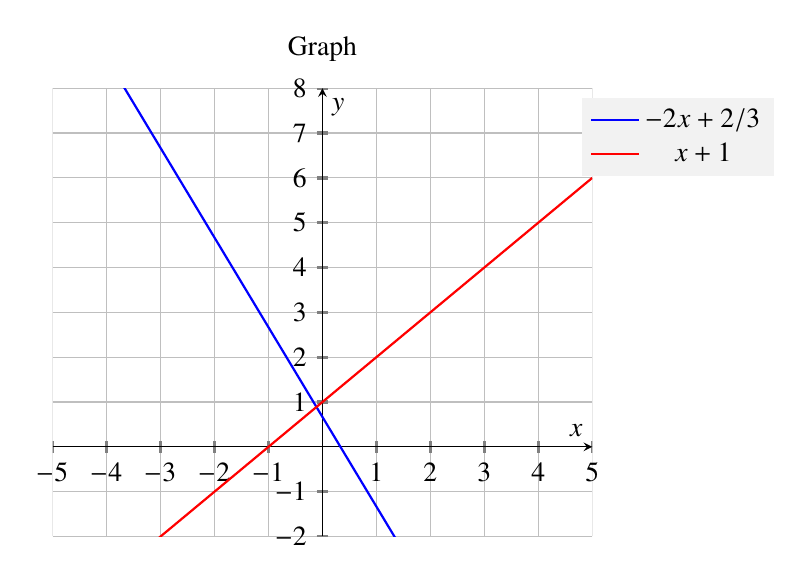
\begin{tikzpicture}
   \begin{axis}[
   legend style={anchor=north west,draw=none,fill=gray!10},
   axis lines=middle,
   grid=major,
   xmin=-5,
   xmax=5,
   ymin=-2,
   ymax=8,
   title=Graph,
   xlabel={$x$},
   ylabel={$y$},
   xtick={-5,-4,...,5},
   ytick={-2,-1,...,8},
   tick style={very thick}
   ]
   \addplot[blue,thick]{-2*x+2/3};
   \addlegendentry{$-2x+2/3$}
   \addplot[red,thick]{x+1};
   \addlegendentry{$x+1$}
   \end{axis}
   \end{tikzpicture}
   \caption{This is a plot of pair of straight lines when k=-3}
   \end{figure}
\begin{figure}
   \centering
   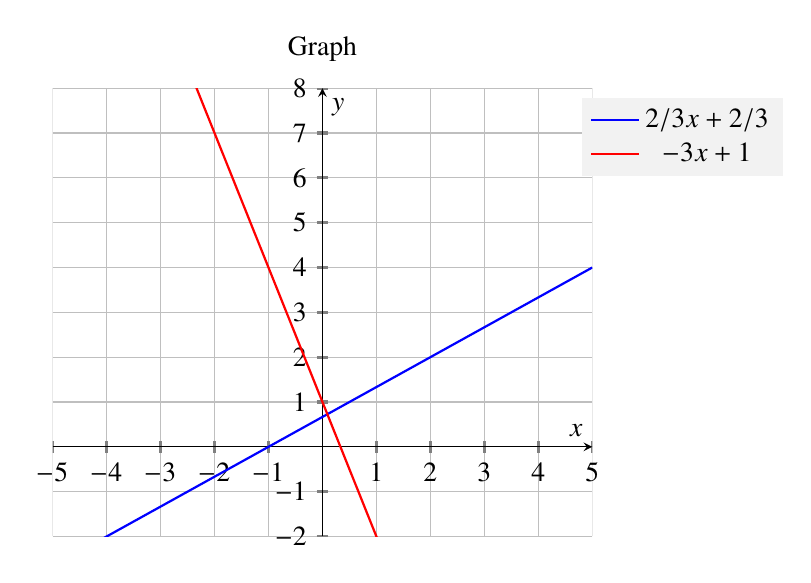
\begin{tikzpicture}
   \begin{axis}[
   legend style={anchor=north west,draw=none,fill=gray!10},
   axis lines=middle,
   grid=major,
   xmin=-5,
   xmax=5,
   ymin=-2,
   ymax=8,
   title=Graph,
   xlabel={$x$},
   ylabel={$y$},
   xtick={-5,-4,...,5},
   ytick={-2,-1,...,8},
   tick style={very thick}
   ]
   \addplot[blue,thick]{2/3*x+2/3};
   \addlegendentry{$2/3x+2/3$}
   \addplot[red,thick]{-3*x+1};
   \addlegendentry{$-3x+1$}
   \end{axis}
   \end{tikzpicture}
   \caption{This is a plot of pair of straight lines when k=-7}
   \end{figure}
\end{document}